
\documentclass[12pt,aspectratio=169]{beamer}

\usepackage[utf8]{inputenc}
\usepackage{libertine}

% Package pour bloc vidéo
\usepackage[absolute,showboxes,overlay]{textpos}
\TPshowboxestrue % commenter une fois fini
%\TPshowboxesfalse % décommenter pour faire disparaitre les boites
\textblockorigin{10mm}{10mm} % origine des positions

\newcommand{\videoblock}{
    \begin{textblock*}{50mm}[0,0](99mm,50mm)
      % \begin{textblock*}{largeur}[ancrage](coordonnées du block)
      { \centering \color{blue}\textbf{Zone Video}}
        \vspace{2.7cm}
    \end{textblock*}
}

\newcommand{\blockgauche}[1]{
	\begin{columns}
		\begin{column}{0.66\textwidth}
		#1
		\end{column}
		\begin{column}{0.33\textwidth}
		\end{column}
	\end{columns}
}

\usetheme{Boadilla}
\usecolortheme{beaver}


\title[Conférence \LaTeX{}]{Comment enregistrer une vidéo-présentation : outils pour une recherche distantielle}
\author{Beamer + Panopto}
\date{\today}


\begin{document}

\begin{frame}

     \titlepage
     \videoblock
\end{frame}

\section{Problème de recherche}


\begin{frame}{Pourquoi donc présenter à distance ?}

Une conférences internationale en 2013 = enrégistrement d'une présentation vidéo+diapos. 

Le temps passé à préparer la vidéo peut se mesurer par une fonction exponentielle. 

Et pourtant... 

\begin{itemize}
\item Plus de réservations d'hôtels, billets de train, remboursements, etc.
\item Plus de travail sur le beamer dans l'avion, ni le soir à l'hôtel.
\end{itemize}

\blockgauche{
\begin{itemize}
\item Plus de ``social events'', mais une meilleure maîtrise de Zoom, Webex, Teams, ... pour tous.
\item Bientôt conférences en réalité virtuelle, puis augmentée.
\end{itemize}

\vspace{-0.5cm}
\hspace{4cm} 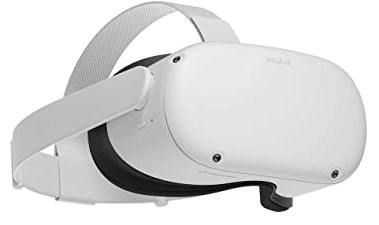
\includegraphics[width=2cm]{quest2.jpg}
}

\videoblock
\end{frame}

\begin{frame}{Ma titre ici}
Contenu de la diapo
\videoblock
\end{frame}

\section{Conclusion}
\begin{frame}{Conclusion}
\videoblock
\end{frame}
 
\end{document}
